\subsection{Сведения о платформе реализации с указанием основных функций операционной системы, необходимых для работы модуля}
\subsection{Обоснование целесообразности разработки оригинальных модулей программного обеспечения}
\subsection{Обоснование выбора технологии программирования и средств разработки}
\subsection{Описание консольного интерфейса программы}% (выбор цветовой палитры экранных форм, расположение элементов управления на них, использование «горячих» клавиш  акселераторов, выпадающих меню и пр.)}
Интерфейс программы представлен в двух реализациях.
Первый — консольная программа в стиле классического Unix. Интерфейс командной строки более гибкий, позволяет выставить необходимые опции/флаги и запустить программу. Особенности в сравнении с графическим интерфейсом:
\begin{itemize}
\item Интерфейс командной строки позволяет писать скрипты для автоматизации запуска и тестирования с различными входными параметрами, что средствами графического интерфейса гораздо сложнее;
\item Большая функциональность;
\item Некая сложность при использовании, неопытным пользователям;
\item Невозможность просмотра выходных результатов.
\end{itemize}

\begin{figure}[ht]
\center{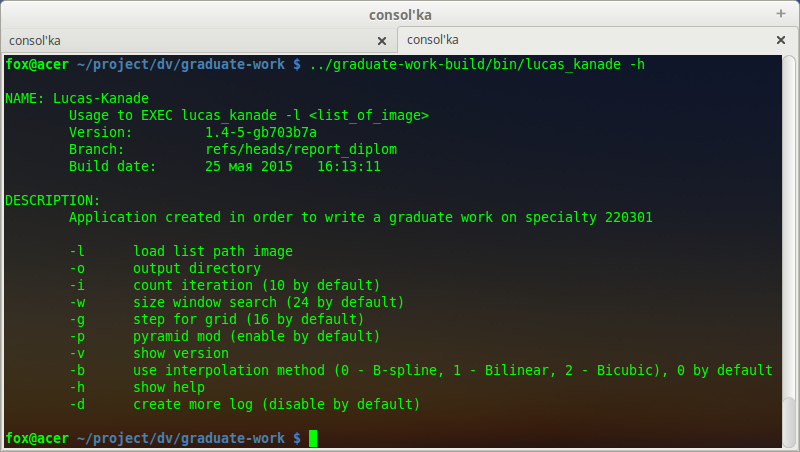
\includegraphics[width=0.8\linewidth]{consol_screen}}
\caption{Пример консольного интерфейса в среде linux}
\label{pic:con_scr}
\end{figure}

\subsubsection{Перечень команд для запуска}
\begin{itemize}
\item l — список изображений для обработки;
\item o — директория для выходных результатов;
\item i — число уточнений при поиске смещённой части (по умолчанию равна 10);
\item w — радиус окна поиска (по умолчанию равна 24);
\item g — шаг между векторами оптического потока(по умолчанию равна 16);
\item p — применить метод пирамиды(по умолчанию опция включена);
\item v — показать версию програмного обеспечения;
\item b — использование метода интерполяции(0 — Б-сплайн, 1 — Билинейная, 2 — Бикубическая), по умолчанию 0;
\item h — показать краткую справку;
\item d — генерировать подробный лог файл(по умолчанию опция выключена).
\end{itemize}
\subsection{Описание графического интерфейса программы}
Второй графический — более удобный для неопытного пользователя. 

\begin{figure}[ht]
\center{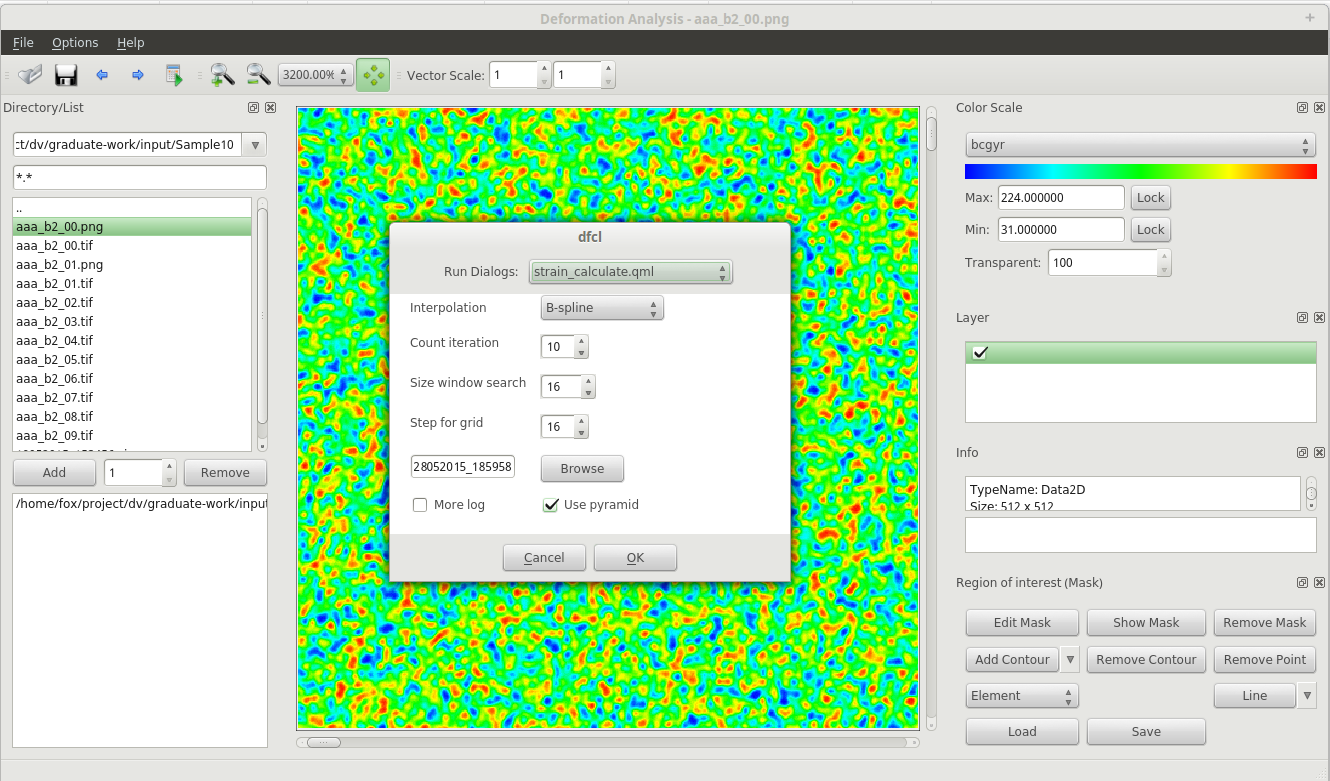
\includegraphics[width=0.8\linewidth]{gui_screen}}
\caption{Пример графического интерфейса}
\label{pic:gui_scr}
\end{figure}

\subsection{Справочную систему пользователя для разрабатываемого модуля,требования к уровню квалификации пользователя}
\subsection{Листинг программы с комментариями, поясняющими работу основных блоков}
\subsection{Блоксхему оригинальных, разработанных автором, алгоритмов работы основных, по мнению автора, программных модулей}
\subsection{Тестовый пример для контроля адекватного функционирования разработанного программного модуля и протокол (листинг) результатов работы программы на этом тестовом примере}